\documentclass[border=10pt]{standalone}
\usepackage[svgnames]{xcolor}
\usepackage{amsmath}
\usepackage{pgfplots}
\pgfplotsset{compat=newest}
\usepackage[sfdefault]{FiraSans}
\usepackage{FiraMono}
\renewcommand*\familydefault{\sfdefault}
\begin{document}
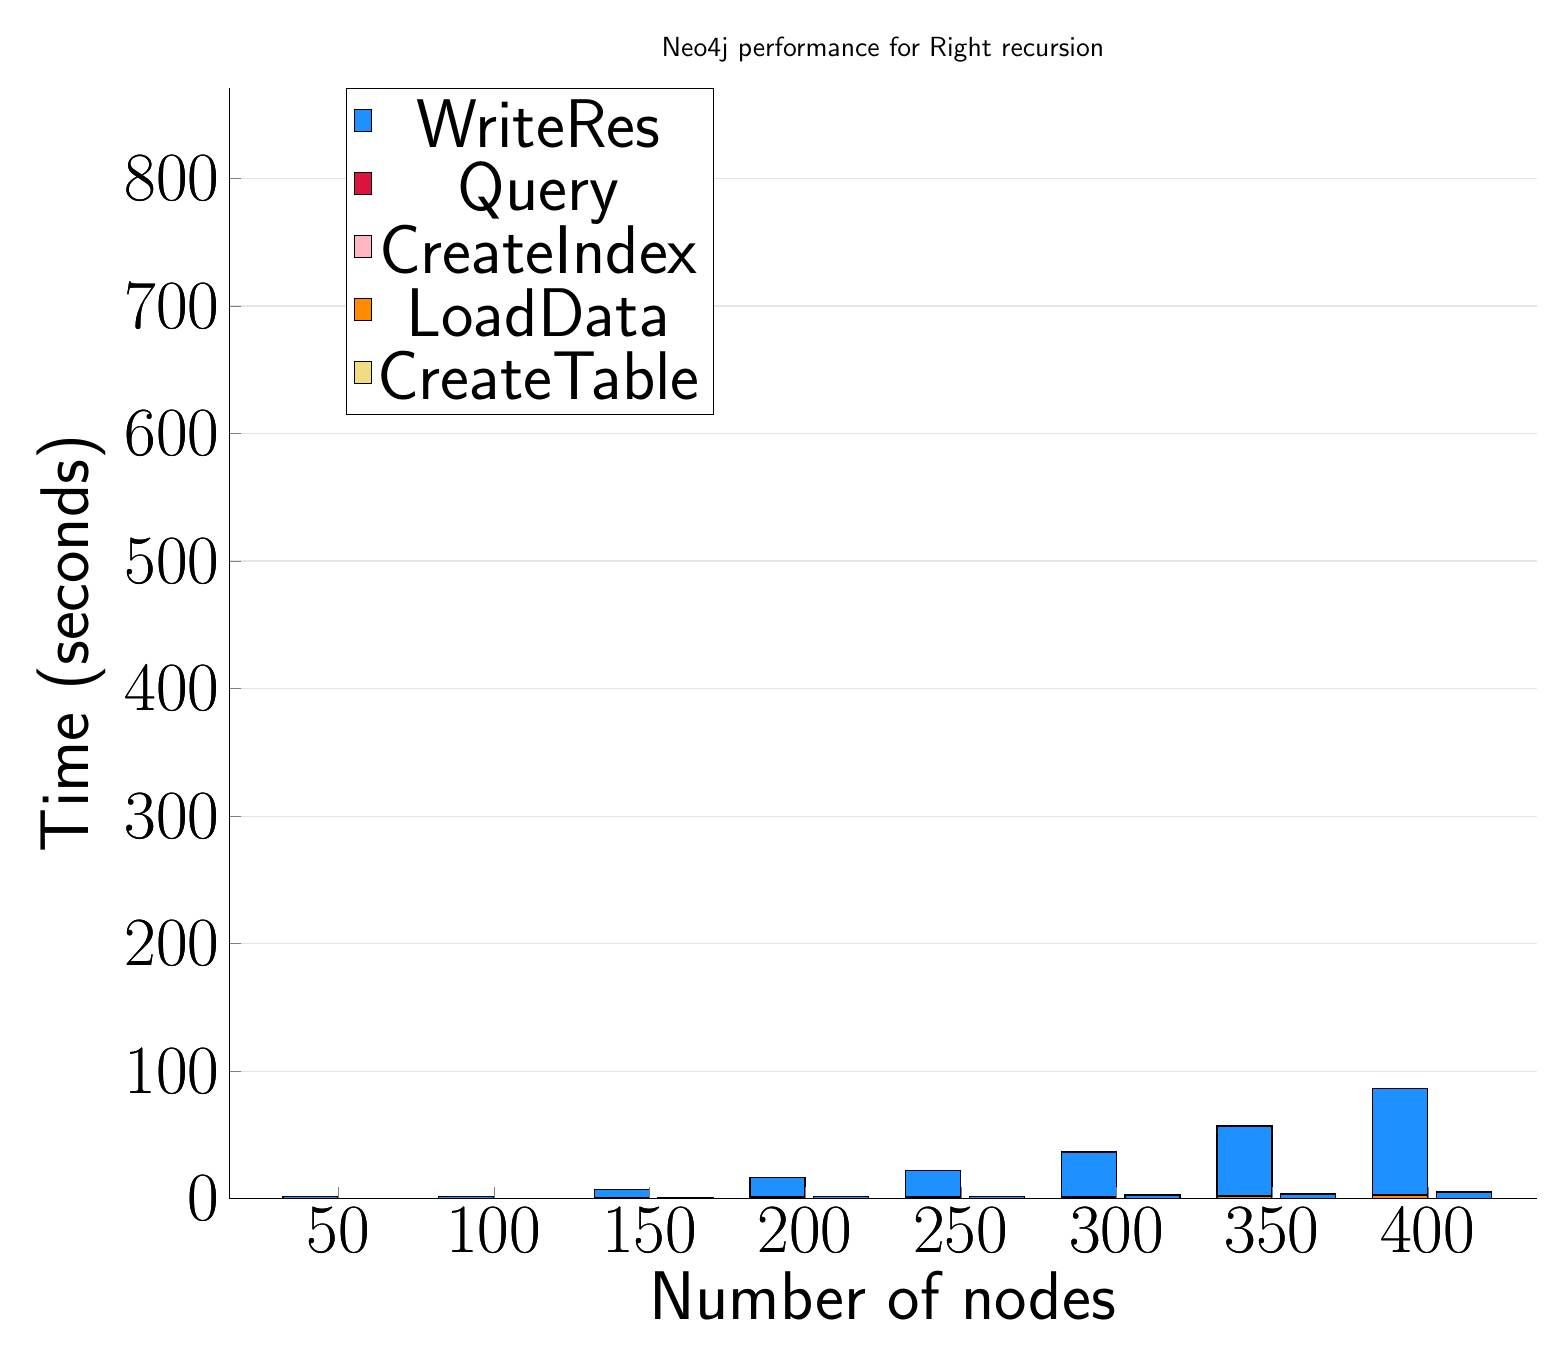
\begin{tikzpicture}
\begin{axis}[
   ybar stacked,
   title={Neo4j performance for Right recursion},
   bar shift=-10pt,
   width=1.5\textwidth,
   bar width=0.7cm,
   ymajorgrids, tick align=inside,
   major grid style={draw=gray!20},
   xtick=data,
   ymin=0, ymax=871.1066666692495,
   axis x line*=bottom,
   axis y line*=left,
   enlarge x limits=0.1,
   legend style={
       at={(0.23, 1)},
       anchor=north,
       legend columns=1,
       font=\Huge,
   },
   ylabel={Time (seconds)},
   xlabel={Number of nodes},
   label style={font=\Huge},
   tick label style={font=\Huge},
]
\addlegendimage{fill=DodgerBlue, draw=black, line width=0.2pt}
\addlegendentry{WriteRes}
\addlegendimage{fill=Crimson, draw=black, line width=0.2pt}
\addlegendentry{Query}
\addlegendimage{fill=LightPink, draw=black, line width=0.2pt}
\addlegendentry{CreateIndex}
\addlegendimage{fill=DarkOrange, draw=black, line width=0.2pt}
\addlegendentry{LoadData}
\addlegendimage{fill=LightGoldenrod, draw=black, line width=0.2pt}
\addlegendentry{CreateTable}
\addplot +[fill=LightGoldenrod, draw=black, line width=0.5pt] coordinates {
    (50, 0.03999999910593033)
    (100, 0.02999999870856603)
    (150, 0.18666666746139526)
    (200, 0.12333333243926366)
    (250, 0.10999999940395355)
    (300, 0.13000000019868216)
    (350, 0.19000000009934107)
    (400, 0.28333333134651184)
};
\addplot +[fill=DarkOrange, draw=black, line width=0.5pt] coordinates {
    (50, 0.14666666587193808)
    (100, 0.14666666835546494)
    (150, 0.5133333330353101)
    (200, 0.9800000016887983)
    (250, 0.9100000013907751)
    (300, 1.2166666661699612)
    (350, 1.6533333336313565)
    (400, 2.2400000020861626)
};
\addplot +[fill=LightPink, draw=black, line width=0.5pt] coordinates {
    (50, 0.07666666805744171)
    (100, 0.08333333084980647)
    (150, 0.20000000049670538)
    (200, 0.33000000069538754)
    (250, 0.30666666726271313)
    (300, 0.39666666835546494)
    (350, 0.5933333337306976)
    (400, 0.6733333319425583)
};
\addplot +[fill=Crimson, draw=black, line width=0.5pt] coordinates {
    (50, 0.03666666646798452)
    (100, 0.01666666567325592)
    (150, 0.003333332637945811)
    (200, 0.1399999981125196)
    (250, 0.003333332637945811)
    (300, 0.003333332637945811)
    (350, 0.07999999821186066)
    (400, 0.003333332637945811)
};
\addplot +[fill=DodgerBlue, draw=black, line width=0.5pt] coordinates {
    (50, 1.5066666652758915)
    (100, 1.4666666686534882)
    (150, 6.376666670044263)
    (200, 14.820000000298023)
    (250, 20.729999999205273)
    (300, 34.74000000208616)
    (350, 54.3233333354195)
    (400, 82.95333333561818)
};
\end{axis}
\begin{axis}[
   ybar stacked,
   bar shift=13pt,
   width=1.5\textwidth,
   bar width=0.7cm,
   ymajorgrids, tick align=inside,
   major grid style={draw=none},
   xtick=data,
   ymin=0, ymax=871.1066666692495,
   axis x line*=none,
   axis y line*=none,
   enlarge x limits=0.1,
   label style={font=\Huge},
   tick label style={font=\Huge},
]
\addplot +[fill=LightGoldenrod, draw=black, line width=0.5pt] coordinates {
    (50, 0.010000000000000009)
    (100, 0.003333333333333337)
    (150, 0.006666666666666672)
    (200, 0.009999999999999969)
    (250, 0.006666666666666668)
    (300, 0.006666666666666668)
    (350, 0.006666666666666672)
    (400, 0.006666666666666672)
};
\addplot +[fill=DarkOrange, draw=black, line width=0.5pt] coordinates {
    (50, 0.0)
    (100, 0.003333333333333337)
    (150, 0.003333333333333336)
    (200, 0.0)
    (250, 0.003333333333333318)
    (300, 0.0)
    (350, 0.0)
    (400, 0.0)
};
\addplot +[fill=LightPink, draw=black, line width=0.5pt] coordinates {
    (50, 0.0066666666666666645)
    (100, 0.003333333333333318)
    (150, 0.0)
    (200, 0.006666666666666636)
    (250, 0.0)
    (300, 0.0)
    (350, 0.006666666666666672)
    (400, 0.003333333333333337)
};
\addplot +[fill=Crimson, draw=black, line width=0.5pt] coordinates {
    (50, 0.003333333333333336)
    (100, 0.0033333333333333184)
    (150, 0.0)
    (200, 0.003333333333333336)
    (250, 0.0)
    (300, 0.003333333333333318)
    (350, 0.0)
    (400, 0.0)
};
\addplot +[fill=DodgerBlue, draw=black, line width=0.5pt] coordinates {
    (50, 0.13333333333333333)
    (100, 0.29333333333333333)
    (150, 0.93)
    (200, 1.6499999999999997)
    (250, 1.8466666666666665)
    (300, 2.7000000000000006)
    (350, 3.73)
    (400, 5.023333333333333)
};
\end{axis}
\end{tikzpicture}

\end{document}
